\chapter{Hydrostatics}
\label{ch:hydrostatics}
\section{Stress}
Let us now get back to the piece of ``slime'' we started the last
lecture with. Consider a small volume element inside the slime. There
are forces acting of this small volume element due to the rest of the
slime. These forces act through the surface of the volume element.
Let us be specific and consider a small box (a rectangular
parallelepiped) of slime with its center at $x,y,z$, lying between 
$x-(1/2)\Delta x $ to $x+(1/2)\Delta x$, 
$y-(1/2)\Delta y$ to $y+(1/2)\Delta y$, and 
$z-(1/2)\Delta z$ to $z+(1/2)\Delta z$.
Consider the face at $x+(1/2)\Delta x$. There is a force by the rest of the
slime acting through this face. Let us call this force
$\ff(x+(1/2)\Delta x,y,z)$. In general, this force can point in
any direction, i.e., it can have all the three components,
$f_x(x+(1/2)\Delta x,y,z)$, $f_y(x+(1/2)\Delta x,y,z)$ and 
$f_z(x+(1/2)\Delta x,y,z)$. The force not only depends on space
(i.e., $x,y,z$) but also which face we are considering. At the same
point $x+(1/2)\Delta x,y,z$ we can consider two different planes,
one perpendicular to the $x$ axis, given by $\Delta y \times \Delta
z$, and another perpendicular to the $z$ axis, given by $\Delta y
\times \Delta x$. The force $\ff$ on these two infinitismal area
elements are clearly different. To emphasize that we label each
component of the force accordingly. Each area element can be uniquely labeled by
the direction of the unit vector normal to it. So the force components
of the force acting at $(x+(1/2)\Delta x,y,z$ on the face of the
cube perpendicular to the $x$ direction is labeled by
$xx$, $xy$ and $xz$. 
\begin{marginfigure}
  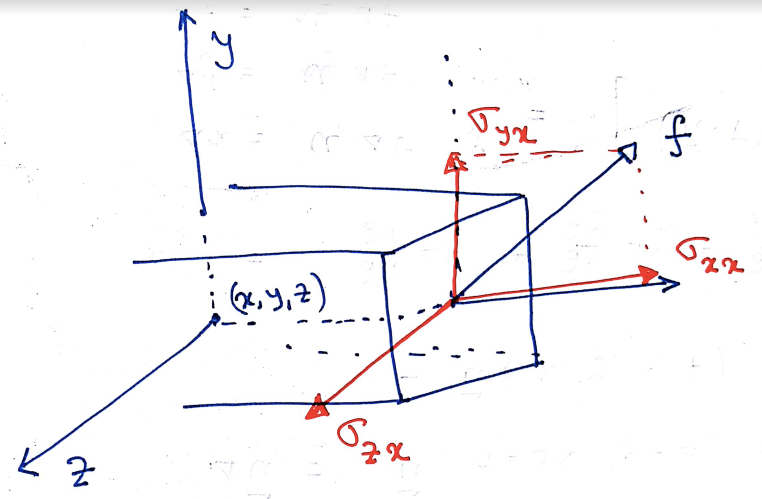
\includegraphics{figures/stress.png}
 \caption{ The force on the face $\Delta y\Delta z$ due to the rest of
 the material is $\ff$. It has components along the three axis,
 $\sigma{xx}$, $\sigma_{yx}$, $\sigma_{zx}$.  If you consider a 
different face at the same point, e.g., $\Delta x\Delta y$, 
the force will be different.}
  \label{fig:stress}
\end{marginfigure}
 Next we define, the force per-unit-area as:
\begin{subequations}
\begin{align} 
\sigma_{xx}(x+(1/2)\Delta x,y,z) \Delta y\Delta z&= f_x(x+(1/2)\Delta x,y,z)\/, \\
\sigma_{yx}(x+(1/2)\Delta x,y,z) \Delta y \Delta z&= f_y(x+(1/2)\Delta x,y,z)\/,
{\rm  and} \\ 
\sigma_{zx}(x+(1/2)\Delta x,y,z) \Delta y \Delta z  &= f_z(x+(1/2)\Delta x,y,z)\/. \end{align}
\end{subequations}
Similarly we can define a set of nine number $\sigma_{\alpha\beta}$.
More compactly, the force acting on an area element $\Delta S$ with
its unit normal $\nhat$ is given by 
\begin{equation}
f_{\alpha} = \sigma_{\alpha\beta}n_{\beta}\Delta S \/.
\end{equation}
As $\ff$ is a vector, by the quotient rule $\sigma_{\alpha\beta}$ is 
a second rank tensor.  This is called the ``stress tensor''.

\begin{fullwidth}
Let us try to calculate the total
force on the volume element $\Delta x\Delta y\Delta z$. 
We have to sum over each component of the
force through all the faces. Let us first sum the  $y$ component along
the two faces perpendicular to the $x$ axis:
\begin{subequations}
\begin{align}
f_y(x+\frac{1}{2}\Delta x,y,z)&+f_y(x-\frac{1}{2}\Delta x,y,z) 
= \left[ \sigma_{yx}(x+(1/2)\Delta x,y,z)-  \sigma_{yx}(x-(1/2)\Delta
  x,y,z) \right] \Delta y\Delta z \nonumber \\
&=\left[ \{\sigma_{yx}(x,y,z) + \partial_x \sigma_{yx}\mid_{x,y,z}\frac{\Delta x}{2} +\ldots\}
            -  \{\sigma_{yx}(x,y,z) - \partial_x
  \sigma_{yx}\mid_{x,y,z}\frac{\Delta x}{2}+ \ldots\}  \right]\Delta y \Delta z
  \nonumber \\
&= \partial_x \sigma_{yx} \Delta x\Delta y\Delta z + \ldots \nonumber \\
\end{align}
\end{subequations} 
\end{fullwidth}
Here we have expanded $\sigma_{yx}$ in a Taylor series and truncated
at the leading order term.  Doing this for all the components over all
the faces, we get the total force $\FF$ on the volume element 
$\Delta V = \Delta x\Delta y\Delta z$ as 
\begin{equation}
F_{\beta} = \partial_{\alpha}\sigma_{\beta\alpha}\Delta V 
\label{A1.2divs}
\end{equation}
%
 \begin{marginfigure}
  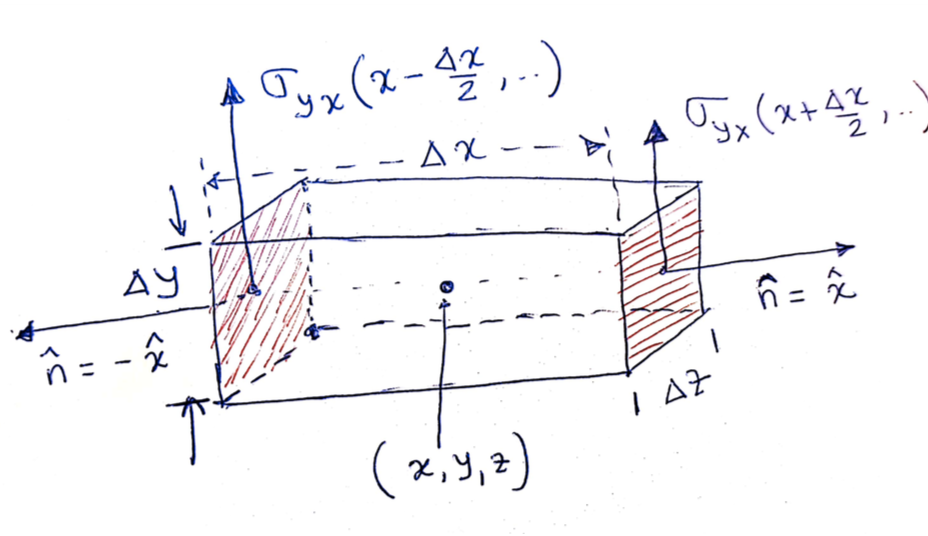
\includegraphics{figures/DivStress.png}
 \caption{ The force on the volume $\Delta x\Delta y\Delta z$ along
   the $y$ direction due to the forces on the two faces that are at
   $x-\Delta x$ and $x+\Delta x$. The force on each face comes from the
   $\sigma_{yx}$  component of the stress multiplied by the 
   area-element  $\nhat\Delta y\Delta z$. The unit vector $\nhat =
   \xhat$ for the face at $x+\Delta x$ and $\nhat=-\xhat$ for the face
 $x-\Delta x$. }
  \label{fig:DivStress}
\end{marginfigure}
%
Here $\FF$ is a vector and $\sigma_{\alpha\beta}$ is a second rank
tensor, then by the quotient rule the components of the operator
$\partial_{\alpha}$ forms a vector, this is the usual gradient
operator 
\begin{equation}
{\bm \nabla} = (\xhat\frac{\partial}{\partial x}+\yhat\frac{\partial}{\partial y}+\zhat\frac{\partial}{\partial z} ) 
\end{equation}
Thus you may think of RHS of \Eq{A1.2divs} as the divergence of the
stress tensor. You need to be careful about one point though, although
the RHS of \Eq{A1.2divs} is often called a divergence it is not a
scalar as usual divergence of a vector field is, but a vector; thus it
is not invariant under rotation. 

By Newton's laws the force $\FF$ is mass times acceleration of the
small volume element $\Delta V$. Let us now associate a density and a
velocity to every point of a deformable body, $\rho(x,y,z)$ and 
$\vv(x,y,z)$.  The equation of motion then becomes
\begin{equation}
\boxed{
\rho\frac{dv_{\alpha}}{dt} = \partial_{\beta}\sigma_{\alpha\beta}
}
\label{A1.2:motion}
\end{equation}

\section{What is a fluid ?}

As the subject of these lectures is \textit{fluid} mechanics I have been
guilty of not even defining what a fluid is. So far I have talked about
kinematics of deformable objects, whatever I have said applies to both
deformable solid -- all solids are deformable -- and fluids. From the
point of view of continuum mechanics -- the view that we adopt in
these lectures -- a fluid is such a material in which at a steady
state the off-diagonal components of the stress tensor must be
zero. This may seem to be a very abstract definition of a fluid, so
let me try to state it more simply. The diagonal components of stress
tensor is  either compressive or extensional. They can either dilate or
compress a material. But an off-diagonal component is a shear.
So the ``definition'' of fluid can be stated simply as: `` under shear,
fluid flows''. Interpreted differently, this is also the simplest
definition of a fluid: `` a fluid at rest always takes the shape of
its container''.  Clearly most materials we consider as fluid, e.g.,  air,
water, wine, oil satisfies this definition. But what about mud or
cement ? It depends on how ``thick'' the mud is and also \textit{ how
  long} you wait till you for it to reach a steady state. Given enough
time -- geological time-scales -- even mountains flow. 
So this definition of fluid depends on the time-scale over which you ask
the question.  Alternatively, we can try to define fluid by its
structure: it is easier to define a solid first. The molecules in a
solid are organized on a regular lattice. By contrast, in a fluid they
are not. But there is something else the behaves like a solid as far
las stresses are concerned but its structure is close to liquids than
to solids : glasses.  Maybe glasses are actually liquids that flows
very very slowly ? Glass windows in old cathedrals are often found to
be uneven, typically thicker at the bottom. But estimates show that 
these are not evidences of flow of glass: `` window glasses may flow 
at ambient temperature only over incredibly long times, 
which exceed the limits of human
history.''\cite{zanotto1998cathedral,zanotto1999cathedral}. 
At the moment, the consensus among scientists is that glass are a
new phase of matter, neither liquids nor solids, but this is still
very much an active field of research. 
To summarize, in the rest of these lectures I shall use the definition of fluid I gave at the
beginning of this section, but be aware that the definition has
nuances. 

\section{Fluid at rest}
By the definition of the fluid at rest, the stress tensor can not have
any off-diagonal component, it must have only diagonal components.
Hence for a fluid 
\begin{equation}
\sigma_{\alpha\beta} = 0 \quad\text{for $\alpha\neq\beta$} 
\label{A1.2:statics}
\end{equation}
The tensor quadratic of this tensor is then an ellipsoid. 
But the expression in \Eq{A1.2:statics} is a physical law, hence must be true in all
coordinate systems, the tensor quadratic must then be a sphere
the only ellipsoid that is invariant under rotation of coordinate
systems. The stress at every point in a fluid at rest can then be
specified by just a single number, 
\begin{equation}
\sigma_{\alpha\beta} = -p \delta_{\alpha\beta}\/,
\label{A1.2:pressure}
\end{equation}
the pressure, a scalar. Note the sign in \Eq{A1.2:pressure}. 
Strictly speaking the the stress can be both positive or negative and
in a solid it can have both signs, but in a liquid the stress is
always a compression. We have emphasized this with the negative sign
in \Eq{A1.2:pressure}. Blaise Pascal, as far as I know, was the first to perceive
this law. This forms the basis of hydraulic press and hydraulic brakes
in cars. We shall not go into the engineering details of a hydraulic
press, I do recomment that you look at the wikipedia page
\url{https://en.wikipedia.org/wiki/Hydraulic_press} and if you enjoy
disaster movies you may like the youtube channel 
\url{https://www.youtube.com/channel/UCcMDMoNu66_1Hwi5-MeiQgw}
where you can see videos of everyday objects being crushed,
pointlessly, in a hydraulic press. 

Notice that so far we have not considered any external forces, e.g,
gravity.  If the force can be obtained as the negative gradient of a potential
$\Phi$, the state of mechanical equilibrium of a fluid
at rest is then given by 
\begin{equation}
-\grad p - \grad \Phi = 0 
\label{A1.2:fstatics}
\end{equation}
\marginnote{
\begin{equation}
\partial_{\alpha}\sigma_{\beta\alpha}
= -\partial_{\alpha}p\delta_{\beta\alpha} = -\grad p \nonumber
\end{equation}
}
This equation can be integrated\footnote{But watch out for what is
  going to come later in section~\ref{sec:multi}.} to obtain 
\begin{equation}
p + \Phi = {\rm constant}
\label{A1.2:pot}
\end{equation}
The constant must be determined from normalization of the potential
and pressure. 

In principle, the story of hydrostatics is now over.  Let us work out
a few illustrative examples.
\subsection{Units, numerical values}
The unit of pressure (or stress in general) is force-per-unit-area,
which in SI units is ${\rm Newton}{\rm meter}^{-2}$ defined to be one
Pascal. The standard atmospheric pressure is $76 {\rm cm}$ mercury.
Consider a column of mercury of height $h = 76 \cm$ and cross-section
$\Delta A$. The gravitational force at the base is $F= h \rho_{\rm
  mercury} g \Delta A$ and the pressure is 
which is 
\begin{eqnarray}
p_{\rm atm} =&\frac{F}{\Delta A} = h\rho_{\rm mercury} g =
76 \times 10^{-2} \meter \times 13.596 \frac{\gram}{\cm^3} \times 10 \frac{\meter}{\sec^2} \nonumber
\nonumber   \\
=&76 \meter\times 10^{-2} \times 13.596 \times \frac{10^{-3}\kg}{10^{-6}
  \meter^3} \times 10 \frac{\meter}{\sec^2} \nonumber \\
=&76\times 13.596\times 10^{2} \frac{\meter^2\kg  }{\meter^3\sec^2}
    \approx 103 {\rm kPa}  \nonumber
\end{eqnarray}
where ${\rm Pa} =  \kg\meter^{-1}\sec^{-2}$. This demonstrates how
small one Pascal is.  The standard atmospheric pressure is about
hundred kilo Pascal ! 
\subsection{Isothermal atmosphere}
Often the external potential comes from gravity, 
\begin{equation}
\Phi = \rho\Psi
\end{equation}
where $\Psi$ is the gravitational potential. 
The simplest problem in this genre is an ideal gas under isothermal
conditions. In the case the ideal gas law tells us $pV = N\kB T$
where $N$ is the total number of molecules in a volume $V$, with
temperature $T$ and the Boltzmann constant $\kB$. This implies,
$p=n\kB T $ where $n=N/V$ is the number of molecules-per-unit-volume. 
Let us assume that the gas is made out of a single type of gas
molecule each of which has mass $m$. Then 
$p=\rho\kB T/m $. Equation~\ref{A1.2:fstatics} then takes the form
\begin{subequations}
\begin{align}
\left(\frac{\kB T}{m}\right)\frac{d}{dz} \rho &= -\rho g  \\
\implies \rho(z) &= \rho(z=0)\exp(-\frac{mgz}{\kB T})
\end{align}
\end{subequations}
The assumption of isothermal atmosphere is not very accurate for our
planet; the actual behavior seen in the atmosphere is somewhat
different as discussed by Falkovich~\cite{Falkovich2018fluid}.
%\subsection{Stability of a boat}
\marginnote{ There are two issues with this Problem~\ref{prb2.1}. First, in the laboratory
  frame of reference this problem is really a problem of dynamics not
  of statics, so this does not belong here. This is true for all
  problems that involve centrifugal forces. Secondly, there is no
  {\textit a priori} reason to think that if you do the experiment you
  shall find the a steady solution even in the frame of the rotating
  bucket. The solution we find may simply be an unstable solution and
  some other physical behavior may be realized. } 
\begin{Exercise}
\Question
\label{prb2.1}
{\bf A bucket rotating about its own axis.}\\
Let us consider a bucket rotating about its own axis -- a
centrifuge. In the frame of the bucket the flow is at rest. What is
the shape of (the surface of) water in the bucket ? \\
Let us use cylindrical coordinate system with the $z$ axis of the
cylindrical coordinate system coinciding with the axis of rotation. 
If the bucket is rotating with an angular velocity $\Omega$, the
centrifugal force, on a volume element of size $\Delta V$ at a 
point ($r,\phi,z$) points in radially outward direction, 
$\FF = \rhat F_{r} = \rhat \rho\Delta V \Omega^2r$. The corresponding
potential is defined to be 
$-\frac{\partial\Phi(r)_{\rm cfg}}{\partial r} =   \rho\Omega^2r$.
The total potential is given by $\Phi(r)_{\rm cfg}$ and the potential
due to gravity, $\Phi_{\rm g}(z)$. The potential appearing in  
 \Eq{A1.2:pot} is the sum of these two potentials.  This gives the
 pressure as a function of $r$ and $z$ including an arbitrary
 constant. The pressure that appears here is the pressure over and
 above the atmospheric pressure which we assume is zero. The equation
 for the free surface is then given by $p(r,z) = 0$. Show that this
 surface is a paraboloid of revolution. 

%\begin{marginfigure}
 % 
\includegraphics{figures/shape_of_water.png}
%\caption{}
%\end{marginfigure}
% 
\Question
{\bf Stress in your bones.} \\
Model your body to be supported two cylindrical pillars which are your
legs. What is the pressure on them at their base ? Now think about a
giant who is $12$ times bigger than you in all directions -- that is
how Gulliver described the Brobdingnags. Estimate the stress suffered
by the bones of those giants. The stress that can break human bones is
estimated to be about $170 {\rm M Pa}$. Can the Brobdingnags have
bones made out of the same material as ours ? What is the stress in
your bones when you jump down from a height of $1\meter$ ?  
\end{Exercise}
\subsection{A multi-valued potential ?}
\label{sec:multi}
I found the following discussion in on page 47-48 in the book by
Sommerfeld\cite{SomII06}. This is so fascinating that I am
going to reproduce this almost verbatim. 
Sommerfeld comments that while integrating \Eq{A1.2:fstatics}
to obtain \Eq{A1.2:pot} it is necessary but not sufficient that the potential $\Phi$
exists, it must also be {\textit single-valued}. He illustrates this
comment by discussing one specific, ingenious problem where the potential is not
single-valued. 

Consider a weakly conducting fluid such as a solution
of copper-sulphate placed in a shallow cylindrical container with
insulating bottom and conducting side walls. A copper wire runs along
the axis of the container. A potential difference of a few volts is
put between the center wire and the side wall so as to maintain a
current flowing from the axis through the fluid and spreading out
towards the wall.
We use a cylindrical coordinate system, $r,\phi,z$ with the $z$ axis
pointing along the axis of the container. 
\begin{marginfigure}
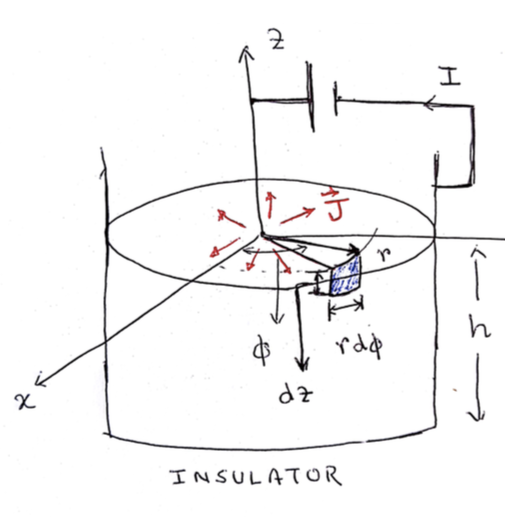
\includegraphics{figures/SomExp.png}
\caption{A sketch of the experiment suggested by Sommerfeld. }
\label{fig:SomExp}
\end{marginfigure}
 Let $I$ be the current in the circuit shown in \Fig{fig:SomExp} and $\JJ$ the vector of
current density pointing radially outward, i.e., $\JJ = J(r)\rhat$. 
The current passing through an element of
area $dS = rd\phi dz$ is given by $JdS$.
 The current and the vector
current density are related by 
\begin{subequations}
\begin{align}
I &= \int_{0}^{h}dz\int_{0}^{2\pi} d\phi J(r) r \\
\implies  \JJ(r) &= \frac{I}{2\pi h r}\rhat
\end{align}
\end{subequations}
where $h$ is the height of the fluid layer. 
We now impose a fairly homogeneous magnetic field $\HH$ 
pointing along the axis of the cylinder. The electromagnetic force
acting upon a fluid element of unit volume is given by 

\begin{equation}
\FF = \JJ \times \HH = \frac{IH}{2\pi r h}\rhat\times\zhat = -\phat \frac{A}{r},
\end{equation}
pointing along the azimuthal direction $\ep$, 
with $A= IH/(2\pi h)$. 
This force has a potential given by 
\begin{subequations}
\begin{align}
-\grad\Phi &= \FF \\
\implies   -\phat\frac{1}{r}\frac{\partial\Phi}{\partial \phi} &= 
-\phat \frac{A}{r} \\ 
\implies \Phi(\phi) &= A\phi
\end{align}
\end{subequations}
\marginnote{
The operator $\grad$ acting on a scalar field $\phi$, 
in cylindrical coordinate system is given by 
\begin{equation}
\grad \phi  = 
(\rhat \partial_r + \phat\frac{1}{r}\partial_{\phi} + \partial_z ) \phi(r,\phi,z)\/.
\end{equation}
One way -- the most straightforward one -- to derive this expression
is to use the chain rule of partial derivatives. We know that in
Cartesian, $\grad\phi$ is given by 
\begin{equation}
\grad \phi = (\eone \partial_1 + \etwo\partial_2 +
\ethree \partial_3)\phi \/.
\label{A1.2:gphi}
\end{equation}
where the Cartesian and the cylindrical coordinate is related by 
\begin{subequations}
\begin{align}
x_1 &= r\cos(\phi) \\ 
x_2 &= r\sin(\phi) \\
x_3 &= z
\end{align}
\end{subequations}
The derivatives in \Eq{A1.2:gphi} can be obtained by 
\begin{equation}
\partial_1 = \frac{\partial r}{\partial x_1}\partial_r 
 +\frac{\partial \phi }{\partial x_1}\partial_{\phi} 
  +\frac{\partial z}{\partial x_1}\partial_z \/,
\end{equation} 
and so on. 
}
Remarkably this potential is not single valued, as
$\phi$ is a multiple valued function, it changes its value by $2\pi A$
for each revolution of the variable $\phi$ about the $z$-axis. 
But hydrostatic pressure must be a single valued function of
position. Hence \Eq{A1.2:pot} cannot be satisfied. This implies that in
this case there is no \textit{hydrostatic} solution to the problem,
the setup will give rise to a flow along the azimuthal direction. 
\section{Stability of hydrostatic solution}
There is one last point to remember. Although it is fairly easy to
obtain a hydrostatics solution it need not always be the solution. For
example consider a pot of water on a stove. Put a few tea leaves in
the water such that you can see what whether the water has a motion or
not. If the heating is very low you shall find all the tea leaves at
the bottom of the pot, but if you touch the top of the surface of the
water you shall find it warm. Heat is being transported through water
but by {\textit conduction}, in the way it is transported through a
solid material. This is a situation in hydrostatics. But if the
heating at the bottom in larger than a threshold, the tea leaves are
set into motion. For a even larger heating you can see bubbles rising
and water boiling. The hydrostatic solution has become {\textit
  unstable} and given rise to motion. This is not the place to go into
the stability problem, we shall spend several lectures on them at a
later stage. 
%----------------------------------------------------------------------------------------
\newpage
\section*{Summary of Act 1}
\begin{thm-non}
The most general motion of a sufficiently small element of a
deformable (i.e., not rigid) body can be represented as the sum of 
\begin{enumerate}
\item a translation
\item a rotation
\item an extension (contraction) in three mutually orthogonal
  directions. 
\end{enumerate}
\end{thm-non}
This is a consequence of a general theorem about tensors:
\begin{thm-non}
Any second rank tensor can be decomposed into one
anti-symmetric and one symmetric tensor.  Any anti-symmetric second
rank tensor can be presented as an (axial) vector. 
\end{thm-non}
The motion of a deformable body, solid or liquid, is given by 
\begin{equation}
\rho\frac{dv_{\alpha}}{dt} = \partial_{\beta}\sigma_{\alpha\beta}
\nonumber
\end{equation}
where $\rho$ is the density, $\vv$ is the velocity with components
$v_{\alpha}$,
and $\sigma_{\alpha\beta}$ is the stress tensor at a point $\rr$. 
\begin{def-non}
The off-diagonal components of the shear stress in a fluid at rest is
zero:
\begin{equation}
\sigma_{\alpha\beta} = 0 \quad\text{for}\quad \alpha \neq \beta \/.
\nonumber
\end{equation}
This is the definition of a fluid.
\end{def-non}
A consequence of this definition is Pascal's law:
\begin{thm-non}
The pressure, on a surface element, at a point in a fluid is a scalar;
i.e., it is the same on all surface elements at that point.  
\end{thm-non}
 If the force on a fluid can be obtained as the negative gradient of a potential
$\Phi$, the state of mechanical equilibrium of a fluid
at rest is then given by 
\begin{equation}
-\grad p - \grad \Phi = 0 
\nonumber
\end{equation}
%----------
